\documentclass[UTF8,a4paper,11pt]{ctexart}

\usepackage[margin=2.4cm]{geometry}
\usepackage{graphicx}
\usepackage{booktabs}
\usepackage{amsmath}
\usepackage{amssymb}
\usepackage{float}
\usepackage{caption}
\usepackage{xcolor}
\usepackage{listings}
\usepackage[numbers]{natbib}
\usepackage[hidelinks]{hyperref}

\pagestyle{plain}
\captionsetup{font=small}
\lstset{
  language=Python,
  basicstyle=\ttfamily\small,
  keywordstyle=\color{blue!70!black},
  commentstyle=\color{green!45!black},
  stringstyle=\color{red!60!black},
  numbers=left,
  numberstyle=\tiny\color{gray},
  frame=single,
  breaklines=true,
  showstringspaces=false,
  columns=fullflexible
}

\title{实验五：神经机器翻译\\[2pt]
\large 从零实现 Encoder--Decoder Transformer（中译英）}
\author{姓名：TODO（由本人填写）\quad 学号：202411581243}
\date{2026 年 11 月}

\begin{document}
\maketitle

\begin{abstract}
本实验用 PyTorch 从零实现了 Encoder--Decoder Transformer，在 9000 对中英平行句对上
训练中译英系统，使用宽度为 5 的 beam search 解码，并用 \texttt{corpus\_bleu} 评测。
模型参数量为 398{,}336，训练 15 个 epoch（4230 步），在单块 GTX 1080 Ti 上耗时 3 分 01 秒，
最佳验证困惑度为 86.87。测试集语料级 BLEU 为 0.0127（beam search）与 0.0156（贪心解码）。
注意力热力图显示模型学到了初步的词级对齐，但由于模型和语料规模很小，译文语义错误很多。
\end{abstract}

\section{数据与实验设置}

\subsection{数据}
课程数据取自 WMT19 中英训练集的 CWMT 部分\citep{barrault2019wmt19}，共
9000/500/500 对训练/验证/测试句对。中文侧不做分词，英文侧已统一小写、标点与词以空格分开。
两种语言各使用一个在训练集上训练的 BPE 分词器\citep{sennrich2016bpe}，词表均为 3200，
特殊符号为 \texttt{<unk>=0}、\texttt{<s>=1}、\texttt{</s>=2}、\texttt{<pad>=3}。
编码时自动在句首、句尾加入 \texttt{<s>} 与 \texttt{</s>}，超过 32 的序列截断并保留
\texttt{</s>}。

\subsection{超参数}
模型与训练超参数严格按实验要求设置，见表~\ref{tab:hparams}。

\begin{table}[H]
\centering
\caption{模型、训练与解码超参数（与实验要求表 1 一致）。}
\label{tab:hparams}
\begin{tabular}{llll}
\toprule
模型 & 取值 & 训练/解码 & 取值 \\
\midrule
隐状态维度 $d$ & 32 & batch 大小 & 32 \\
FFN 中间维度 $d_I$ & 128 & 优化器 & Adam（默认 betas） \\
注意力头数 $H$ & 4 & 学习率 & $10^{-3}$ \\
编码器/解码器层数 & 3 / 3 & epoch 数 & 15 \\
最大序列长度 $N$ & 32 & 打印训练损失 & 每 10 步 \\
hidden dropout & 0.1 & 验证集评估 & 每 100 步 \\
注意力/嵌入 dropout & 无 & beam 宽度 & 5 \\
归一化位置 & post-norm & 最大解码长度 & 32 \\
权重共享 & 无 & 随机种子 & 42 \\
\bottomrule
\end{tabular}
\end{table}

\section{模型实现}

\subsection{多头注意力：避免 Python 循环}
设 batch 大小为 $B$、查询长度为 $T_q$、键长度为 $T_k$、隐维度为 $d$、头数为 $H$，
每个头维度 $d_H=d/H$。实现时先用一个线性层把 $X\in\mathbb{R}^{B\times T\times d}$
投影为 $Q,K,V$，再通过
\[
(B,T,d)\xrightarrow{\text{view}}(B,T,H,d_H)
\xrightarrow{\text{transpose}}(B,H,T,d_H)
\]
把最后一维切成 $H$ 段。随后一次矩阵乘法同时算出所有头的打分：
\[
S = \frac{QK^{\top}}{\sqrt{d_H}}\in\mathbb{R}^{B\times H\times T_q\times T_k}.
\]
掩码在头维度上广播，不需要复制 $H$ 份；softmax 后与 $V$ 相乘，得到
$(B,H,T_q,d_H)$，再 \texttt{transpose} 回 $(B,T_q,H,d_H)$ 并 \texttt{view} 成
$(B,T_q,d)$，最后过输出投影。整个过程中没有对注意力头写 Python 循环。
关键代码如下（\texttt{nmt/model.py}）：

\begin{lstlisting}
q = self._split_heads(self.q_proj(query))   # (B, H, T_q, d_H)
k = self._split_heads(self.k_proj(key))     # (B, H, T_k, d_H)
v = self._split_heads(self.v_proj(value))   # (B, H, T_k, d_H)

scores = torch.matmul(q, k.transpose(-2, -1)) * self.scale
if mask is not None:
    mask = mask.to(torch.bool)
    if mask.dim() == 2:
        mask = mask[:, None, None, :]        # (B, 1, 1, T_k)
    elif mask.dim() == 3:
        mask = mask[:, None, :, :]           # (B, 1, T_q, T_k)
    scores = scores.masked_fill(~mask, torch.finfo(scores.dtype).min)

attn = F.softmax(scores, dim=-1)
context = torch.matmul(attn, v)              # (B, H, T_q, d_H)
context = context.transpose(1, 2).contiguous().view(B, T_q, d)
return self.out_proj(context), attn
\end{lstlisting}

\texttt{forward} 返回 \texttt{(out, attn)}，其中 \texttt{attn} 的形状为
\texttt{(batch\_size, num\_heads, num\_query\_tokens, num\_key\_tokens)}，满足题目要求。

\subsection{两种掩码的构造与合并}
掩码统一约定为 BoolTensor，\texttt{True} 表示“可以注意”。

\begin{itemize}
  \item \textbf{源端 \texttt{<pad>} 掩码}：\texttt{src\_ids.ne(3).unsqueeze(1)}，形状
        $(B,1,T_s)$，pad 列在 softmax 前被置为极小值，权重为 0。
  \item \textbf{解码器因果掩码}：\texttt{torch.tril(ones(T,T))}，形状 $(1,T_t,T_t)$，
        位置 $i$ 只能看到 $j\le i$。
  \item \textbf{解码器合并掩码}：目标端 pad 掩码 $(B,1,T_t)$ 与因果掩码
        $(1,T_t,T_t)$ 做逻辑与，得到 $(B,T_t,T_t)$，同时屏蔽 pad 与未来位置。
\end{itemize}

\begin{lstlisting}
def combine_masks(pad_mask, causal_mask):
    if pad_mask.dim() == 3:
        pad_mask = pad_mask[:, 0, :]                 # (B, T_k)
    return pad_mask.unsqueeze(1) & causal_mask.to(pad_mask.device)
\end{lstlisting}

\texttt{cross-attention} 只使用源端 pad 掩码：查询是解码器隐状态，键/值是编码器输出。
注意被屏蔽的位置用 \texttt{torch.finfo(dtype).min} 而不是 \texttt{-inf}，避免整行被
屏蔽时 softmax 出现 NaN。

\subsection{嵌入、Transformer 块与整体模型}
嵌入层把词嵌入与可学习的位置嵌入相加，编码器和解码器各有一套独立的词嵌入与位置嵌入。
\texttt{TransformerBlock} 用 post-norm：
$\mathrm{LN}(h+\mathrm{Dropout}(\mathrm{Sublayer}(h)))$；解码器块比编码器块多一个
cross-attention 子层。FFN 为 $W^{(2)}\mathrm{ReLU}(W^{(1)}h)$，中间维度 128。
输出层是单独的线性投影，与解码器词嵌入不共享权重。

\section{自检结果（题 a-3）}

运行 \texttt{python nmt/sanity\_check.py} 得到图~\ref{fig:sanity}。程序检查了三种注意力
的输出/权重形状、每行权重之和为 1、以及被屏蔽位置的权重为 0，全部通过。

\begin{figure}[H]
  \centering
  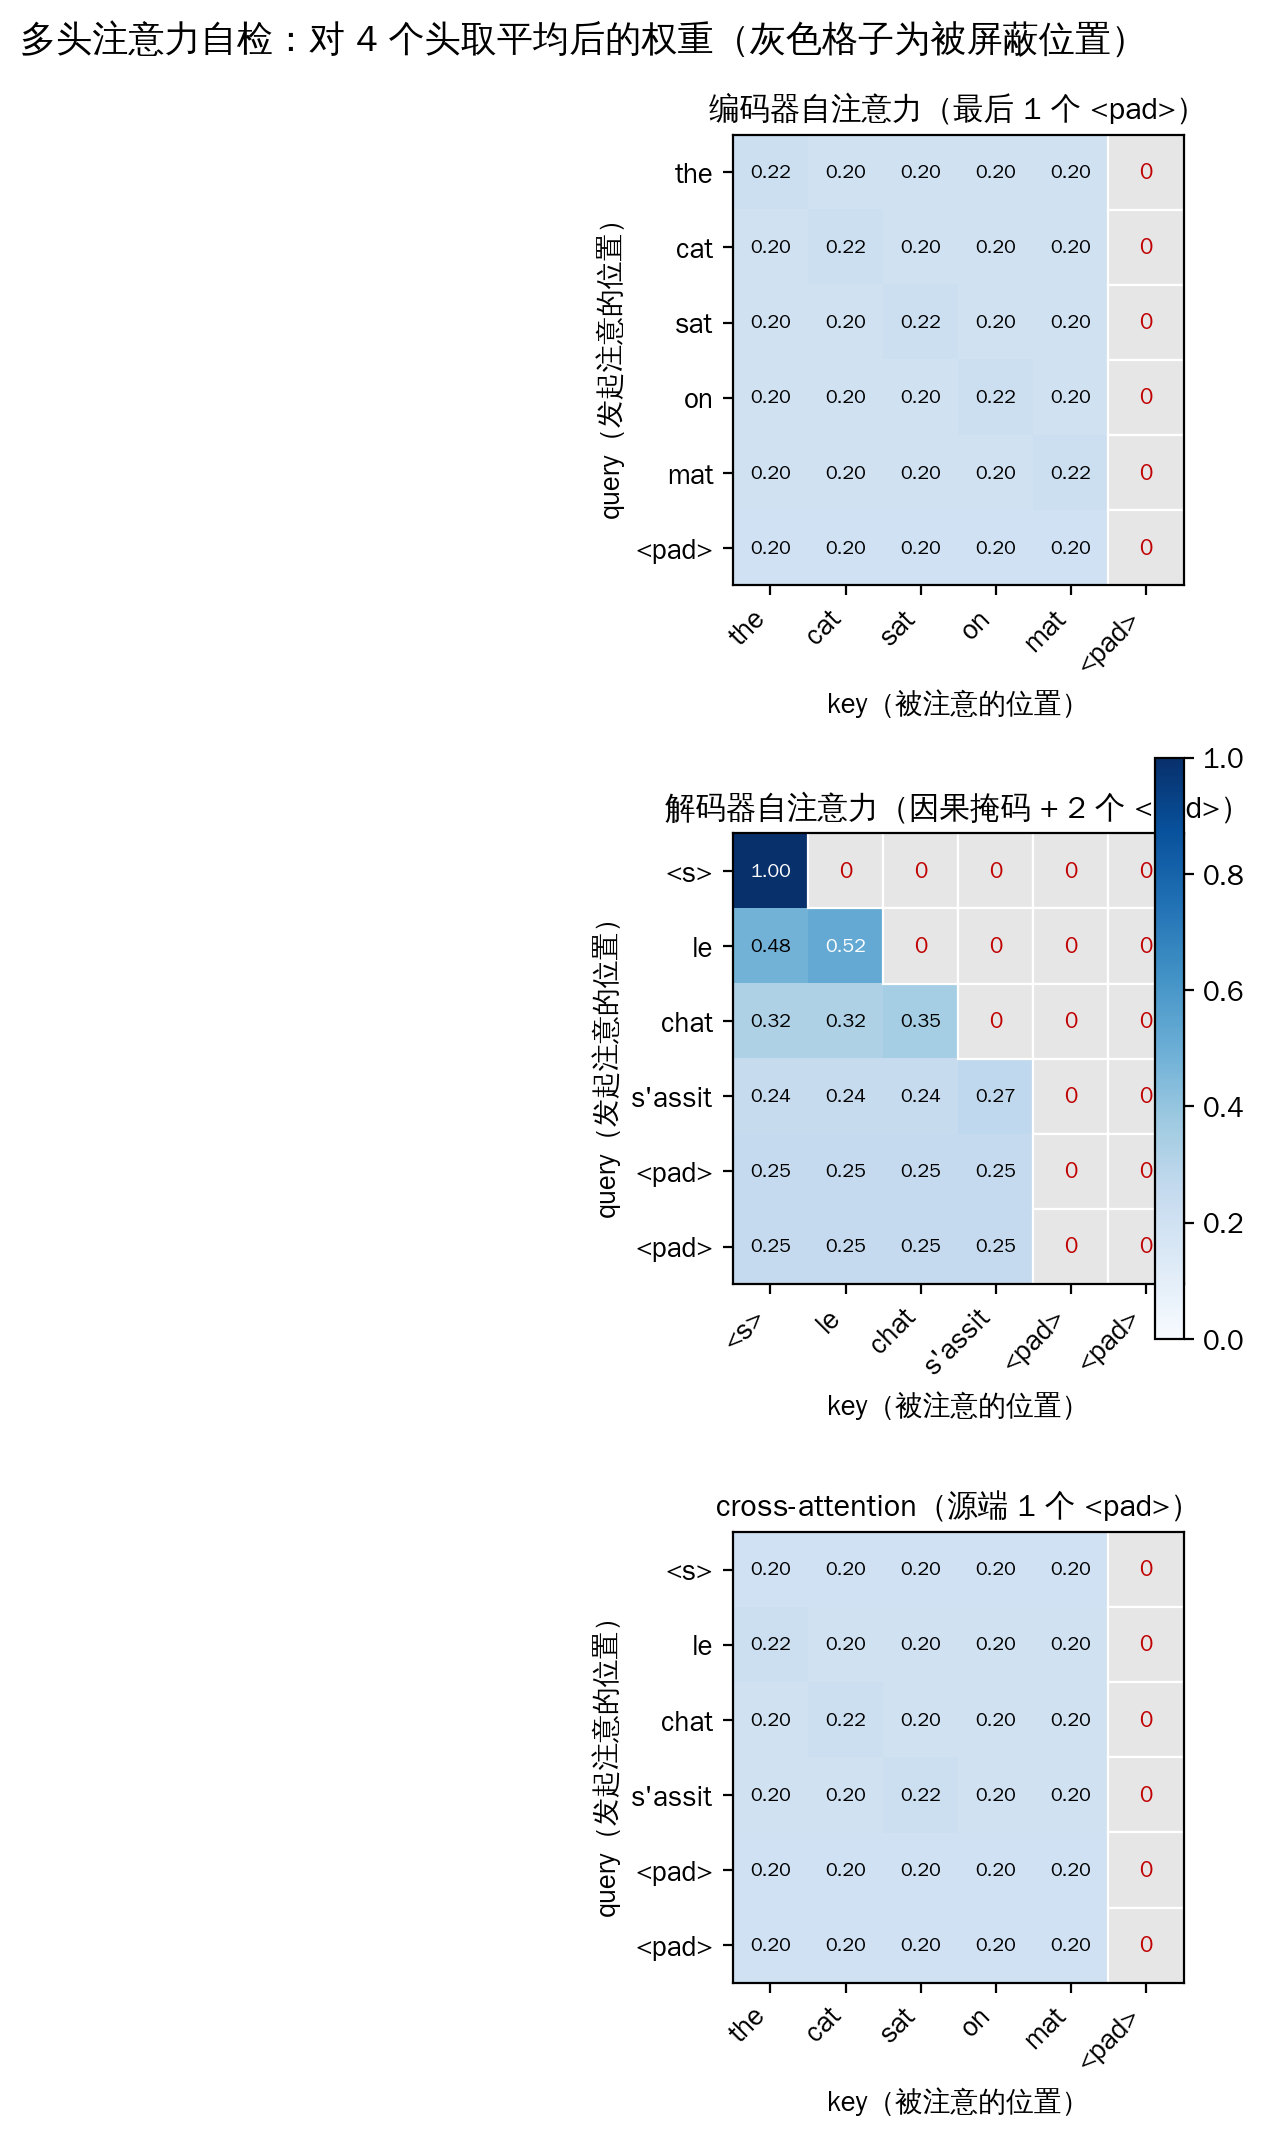
\includegraphics[width=0.86\textwidth]{../nmt/figures/sanity_attention.png}
  \caption{多头注意力自检（4 个头取平均）。灰色格子并标红 0 的位置为被屏蔽位置。}
  \label{fig:sanity}
\end{figure}

逐图说明应为 0 的位置及原因：
\begin{itemize}
  \item \textbf{编码器自注意力}（上）：编码器输入最后一个 token 是 \texttt{<pad>}，
        因此所有 query 行在最后一列（\texttt{<pad>} 作为 key）上的权重都必须为 0，
        否则 pad 会影响上下文表示。
  \item \textbf{解码器自注意力}（中）：最后两个 token 是 \texttt{<pad>}，所以最后两列
        全为 0；同时因果掩码要求 $j>i$ 的上三角全为 0，因此位置 $i$ 只能看到
        $0,\dots,i$。图中同时能看到阶梯状的因果结构和右侧两条空白 pad 列。
  \item \textbf{cross-attention}（下）：键来自编码器，最后一个源 token 是
        \texttt{<pad>}，所以最后一列全为 0；查询侧是解码器，没有因果限制，各行可以
        看到所有非 pad 源位置。
\end{itemize}
注意 pad 作为 query 的行仍然对合法的 key 有归一化权重（行和为 1），这是正常的：
掩码屏蔽的是“被注意的 key”，而不是“发起注意的 query”。

\section{训练（题 b）}

\subsection{损失与困惑度}
训练使用 teacher forcing：解码器输入 \texttt{tgt\_ids[:, :-1]}，预测目标
\texttt{tgt\_ids[:, 1:]}，交叉熵的 \texttt{ignore\_index=3} 排除 \texttt{<pad>}。
验证困惑度按真实目标 token 数加权：
\begin{equation}
  \mathrm{PPL}=\exp\left(\frac{\sum_{\text{batch}}\sum_{t}\ell_t}
  {\sum_{\text{batch}} n_{\text{tok}}}\right).
\end{equation}

\subsection{训练过程}
在 \texttt{gputest12} 的 NVIDIA GeForce GTX 1080 Ti（11 GiB，驱动 535.230.02，
CUDA 12.2，PyTorch 2.5.1+cu121）上训练。共 4230 步，耗时 3 分 01 秒。
训练日志提交在 \texttt{nmt/results/train.log}，损失曲线见图~\ref{fig:loss}。

\begin{figure}[H]
  \centering
  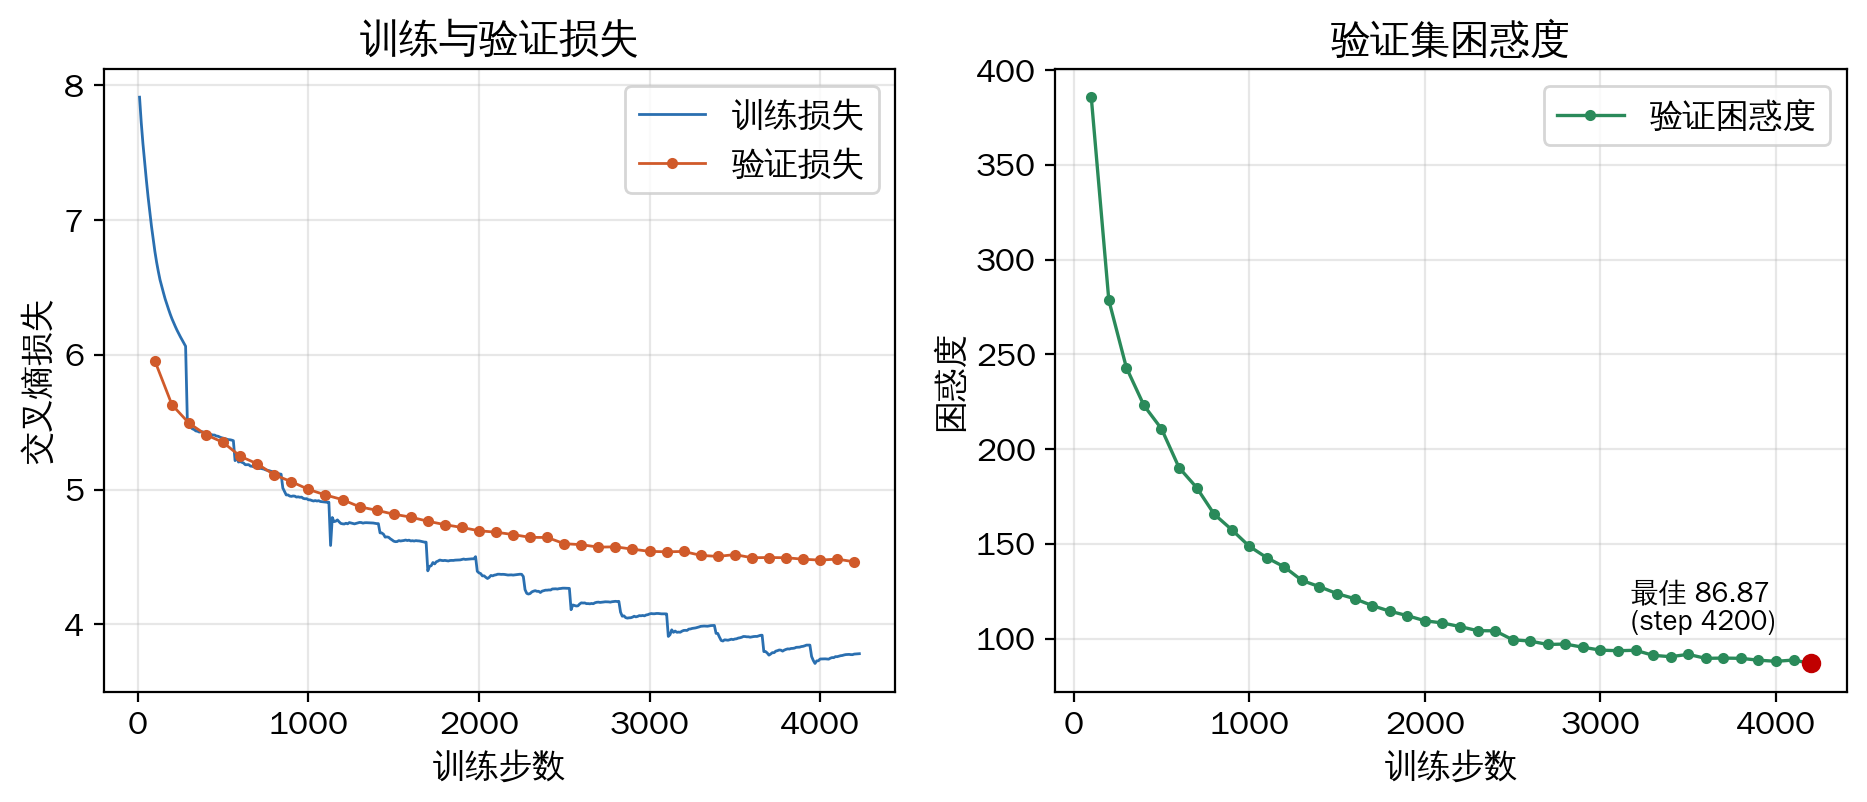
\includegraphics[width=\textwidth]{../nmt/figures/loss_curve.png}
  \caption{训练/验证损失与验证困惑度。红线标出最佳验证困惑度 86.87（第 4200 步）。}
  \label{fig:loss}
\end{figure}

训练损失从约 7.9 降到 3.78，验证损失在前半程快速下降，随后缓慢改善并在第 4200 步
达到最低困惑度 86.87。训练损失仍低于验证损失，说明这个约 40 万参数的小模型在 9000 对
数据上已经出现一定过拟合；继续训练带来的验证收益很小。

\subsection{词表与 batch 统计（题 b）}
运行 \texttt{python nmt/batch\_stats.py}，结果保存在
\texttt{nmt/results/batch\_stats.json}：
\begin{itemize}
  \item[(i)] 源语言（中文）词表大小 \textbf{3200}，目标语言（英文）词表大小
        \textbf{3200}，均含 4 个特殊符号。
  \item[(ii)] 一个训练 batch（32 句）平均有 \textbf{372.03} 个源语言真实 token、
        \textbf{376.63} 个目标语言真实 token。补齐后平均槽位数为 596.91 与 536.43，
        因此 \texttt{<pad>} 在源端平均占 \textbf{37.67\%}，在目标端占 \textbf{29.79\%}。
\end{itemize}
源端 pad 比例更高，是因为中文句子长度差异更大，一个 batch 内按最长句补齐会产生较多填充。

\section{评测与错误分析（题 c）}

\subsection{BLEU}
运行 \texttt{python nmt/evaluate.py} 加载最佳模型，用宽度 5 的 beam search 翻译测试集
500 句，再用 \texttt{nltk.translate.bleu\_score.corpus\_bleu} 计算语料级 BLEU。
结果见表~\ref{tab:bleu}。BLEU 的输入是 detokenize 后的英文句子按空格切分，而不是 BPE token。

\begin{table}[H]
\centering
\caption{测试集 BLEU 与解码耗时（500 句）。}
\label{tab:bleu}
\begin{tabular}{lccc}
\toprule
解码方式 & beam 宽度 & BLEU & 耗时 \\
\midrule
Beam search & 5 & 0.0127 & 23.5 s \\
贪心解码 & -- & 0.0156 & 17.9 s \\
\bottomrule
\end{tabular}
\end{table}

BLEU 很低，符合实验说明中对这个小模型、小数据的预期。有意思的是贪心解码略高于
beam search：由于模型欠拟合且 beam 用长度归一化选句，宽度 5 并不保证语料级 BLEU 更高；
这也说明在模型很弱时，解码策略的收益有限。

\subsection{译文质量与常见错误}
人工查看 \texttt{nmt/results/translations\_beam.txt} 中的译文，可以得到以下观察：
\begin{itemize}
  \item 大多数输出是\textbf{形式合乎语法}的英语短句，词序、冠词和标点基本正常，
        例如 “now , it is not a little boy .”；但语义经常与源句无关。
  \item \textbf{高频模板复用}：模型大量生成 “there are \dots”、“i hope \dots”、
        “she is a very important \dots” 等训练集中常见的句型，把源句内容替换成
        高频词，说明它主要学到了目标语言的局部语言模型，而不是稳定的翻译对应。
  \item \textbf{词义与实体错误}：如 “费用中包括税金。” 译为
        “there are a new york .”，“她教图画课。” 译为 “she is a very important .”，
        内容词大量丢失。
  \item \textbf{短语/习语错误}：“现在有点忙，下次聊天。再见。” 只译出前半句的一部分，
        后半句信息被丢弃；复杂句（含条件从句）只保留了 “if you are \dots” 的框架。
  \item \textbf{长度与截断}：少数译文在 32 个 token 内没有结束，或在语义未完成时输出句号。
\end{itemize}
这些错误与数据规模（9000 对）、模型容量（$d=32$，约 40 万参数）以及中英语序差异大
都有关系；实验要求不通过调超参数来提高 BLEU，因此本文保留上述设置。

\section{Cross-attention 可视化（题 d）}

运行 \texttt{python nmt/visualize\_attention.py}，取最后一个解码器层的 cross-attention，
对 4 个头取平均。图~\ref{fig:attn1} 与图~\ref{fig:attn2} 分别是两个指定例句的贪心解码结果；
行是生成的英文 token，列是中文源 token。两份数值记录在
\texttt{nmt/results/attention\_1.txt} 与 \texttt{attention\_2.txt}。

\begin{figure}[H]
  \centering
  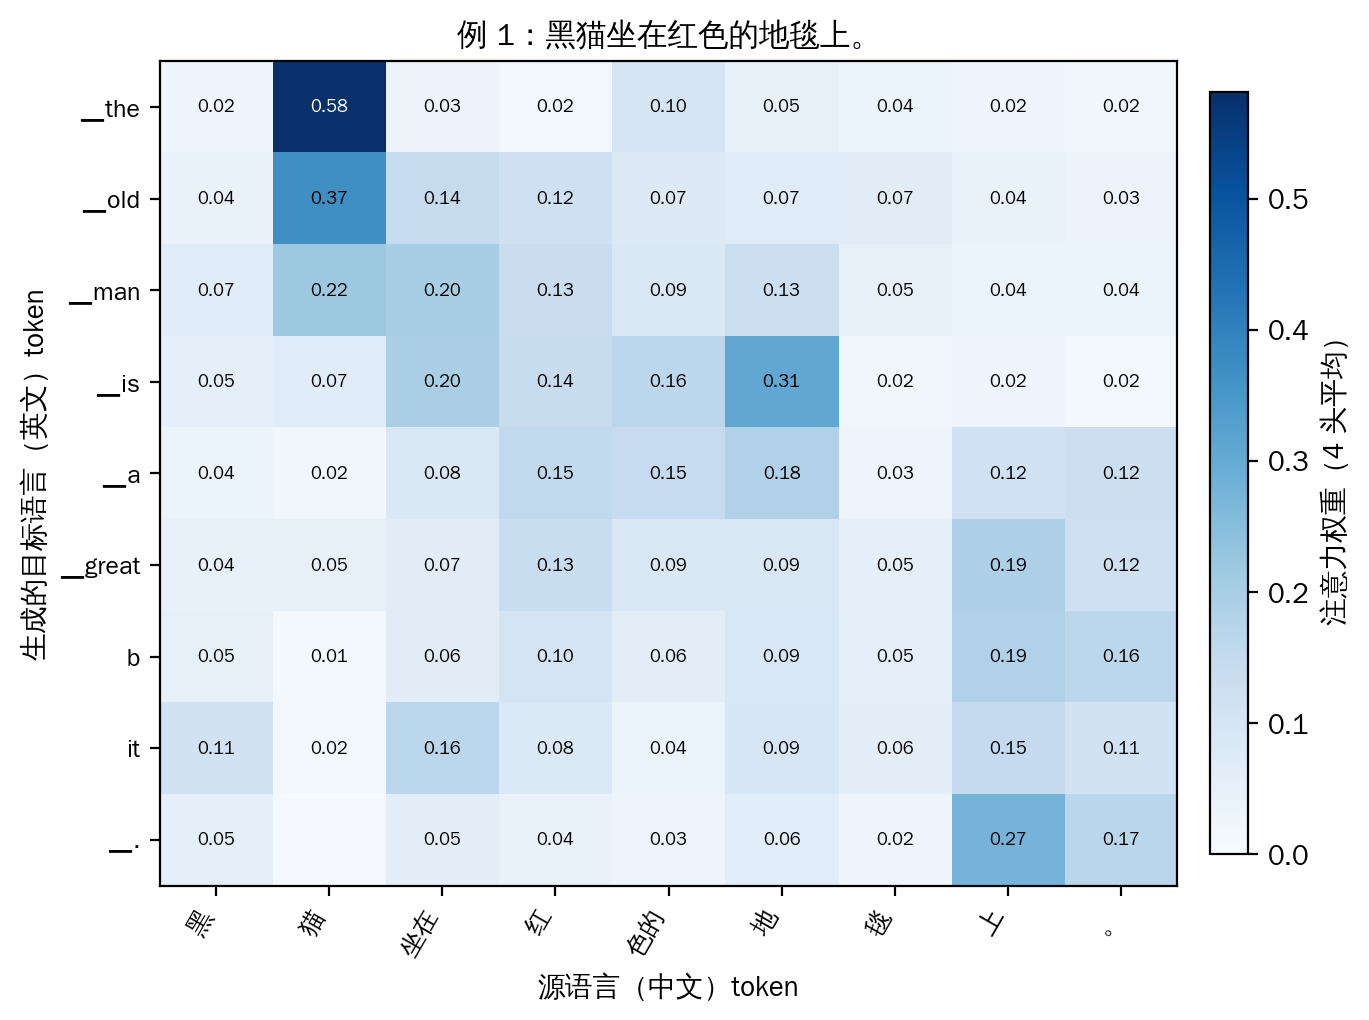
\includegraphics[width=0.92\textwidth]{../nmt/figures/attention_1.png}
  \caption{例 1“黑猫坐在红色的地毯上。”的 cross-attention。译文：
  “the old man is a greatbit .”}
  \label{fig:attn1}
\end{figure}

\begin{figure}[H]
  \centering
  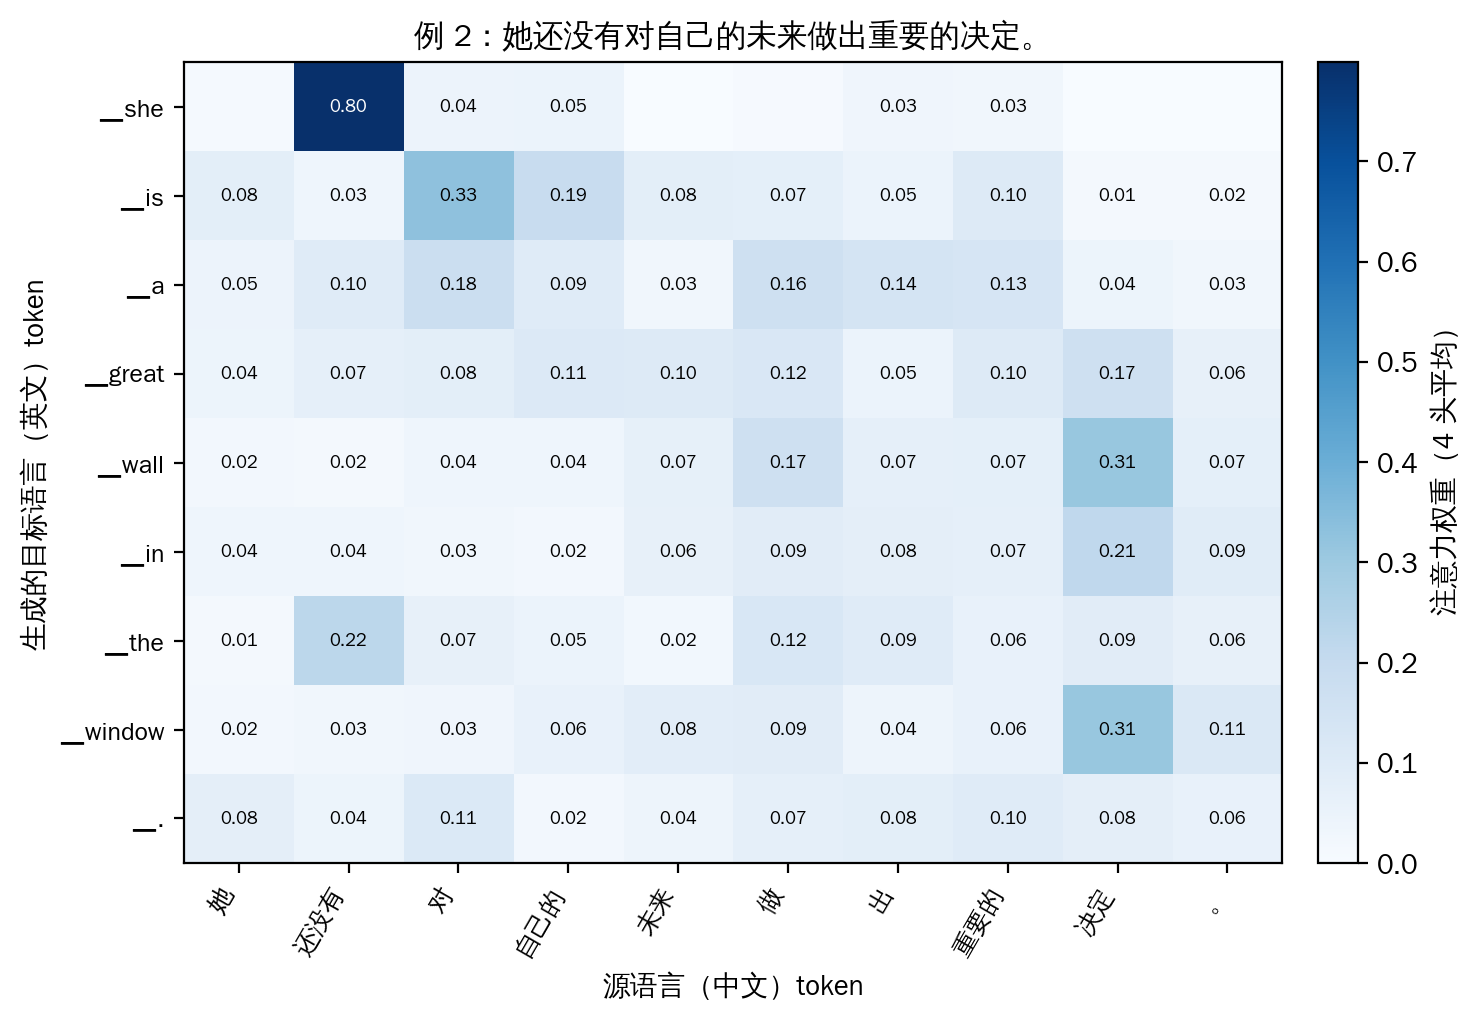
\includegraphics[width=0.92\textwidth]{../nmt/figures/attention_2.png}
  \caption{例 2“她还没有对自己的未来做出重要的决定。”的 cross-attention。译文：
  “she is a great wall in the window .”}
  \label{fig:attn2}
\end{figure}

\subsection{例 1：黑猫坐在红色的地毯上}
译文是 “the old man is a greatbit .”，语义完全错误，但注意力并非随机：
\begin{itemize}
  \item 生成 “the” 与 “old” 时，注意力分别有 0.58 与 0.37 集中在“猫”上，说明模型
        至少把句首的主语名词与译文的第一个名词短语联系了起来，尽管它把“黑猫”错译成
        “old man”。
  \item “is” 在“坐在”上有 0.20，在“毯”上有 0.31，对应“坐在……上”的处所结构；
        “a” 的注意力较分散（最大 0.18），符合冠词没有直接源词对应的特点。
  \item 后半段 “great”“b”“it” 的注意力分散在“红/色的/地/毯/上”多个 token 上，
        没有形成清晰的一对一映射；最后一个句号有 0.27 落在“上”、0.17 落在“。”，
        说明标点和句末位置也被模型当作结束信号。
\end{itemize}
偏离对角线的主要原因是译文本身错了：一旦模型选择了错误的英文词，后续 query 就找不到
稳定的源端对应，注意力只能摊在相邻的内容词上。另一方面，中文“红色的地毯”被 BPE 切成
“红/色的/地/毯”，一个英文词可能对应多个源子词，也会让热力图出现一对多的模糊块。

\subsection{例 2：她还没有对自己的未来做出重要的决定}
译文是 “she is a great wall in the window .”，但第一人称代词的对齐非常清楚：
\begin{itemize}
  \item “she” 有 0.80 的权重集中在“她”上，这是全图最强的对角对齐，说明模型学会了
        主语代词“她→she”。
  \item “is” 的注意力分散到“对”（0.33）与“自己的”（0.19）；“a” 分散在“对/做/出/
        重要的/决定”上，权重大约 0.1--0.18，说明系动词和冠词没有明确的源端对应。
  \item “wall” 与 “window” 各有 0.31 集中在“决定”上；“in” 有 0.21 在“决定”上。
        模型把“决定”错译成名词 “wall/window”，随后把介词短语放在它后面，注意力仍然
        回到这个名词附近，形成了“英文介词短语紧邻名词”的模式。
\end{itemize}
这个例子正好对应中英语序差异。中文的介词短语“对自己的未来”位于动词“做出”之前，
英语通常说 “make an important decision about her own future”，介词短语在名词之后。
图中 “in” 没有去看“未来”，而是看“决定”，说明模型只学到了“介词短语应靠近名词”的
位置习惯，却没有学到“about/in 应指向未来”的语义关系；也就是说，它部分适应了语序，
但没有建立正确的论元对应。四个头平均后，一些可能专门关注“未来”的头被平均掉了，
这也是热力图偏平滑的原因之一。

\subsection{注意力是否揭示模型的处理方式}
两张图都显示：开头的主语/代词位置注意力最集中，随后迅速变得分散。这与译文质量一致：
模型对句首成分较有信心，对后半句的内容词缺乏把握，只能依赖目标语言的常见搭配。
当译文错误时，热力图不会呈现整齐的对角线，而是出现“整行摊平”或“多个英文词共同看同一个
源词”的模式。因此，注意力可以作为诊断工具，但不能单独证明模型“理解”了句子。

\section{复现与耗时}
在仓库根目录依次运行：
\begin{lstlisting}[language=bash,numbers=none]
python nmt/sanity_check.py
python nmt/train.py
python nmt/plot_curve.py
python nmt/batch_stats.py
python nmt/evaluate.py
python nmt/evaluate.py --greedy
python nmt/visualize_attention.py
\end{lstlisting}

\begin{table}[H]
\centering
\caption{各脚本耗时（GTX 1080 Ti，batch 32）。}
\label{tab:time}
\begin{tabular}{lc}
\toprule
脚本 & 耗时 \\
\midrule
\texttt{sanity\_check.py} & $<2$ s \\
\texttt{train.py}（15 epoch，4230 步） & 3 min 01 s \\
\texttt{plot\_curve.py} & $<1$ s \\
\texttt{batch\_stats.py} & 约 8 s \\
\texttt{evaluate.py}（beam，500 句） & 23.5 s \\
\texttt{evaluate.py --greedy} & 17.9 s \\
\texttt{visualize\_attention.py} & 约 3 s \\
\bottomrule
\end{tabular}
\end{table}

服务器与 GPU：\texttt{gputest12}，NVIDIA GeForce GTX 1080 Ti（GPU 0，11 GiB），
驱动 535.230.02，CUDA 12.2。运行环境为 Python 3.10.21、PyTorch 2.5.1+cu121、
transformers 4.57.6、nltk 3.10.4。

\bibliographystyle{plain}
\bibliography{refs}

\appendix
\section{AI 工具使用说明}

\subsection*{使用的提示词}
本次实验使用了支持代码编辑与终端执行的 AI 助手，主要提示词如下（按时间顺序）：
\begin{enumerate}
  \item “按照实验要求以及严格按照 skill 的步骤完成实验，数据集在
        \texttt{/home/s202411581243/workspace/shittt/shit/data}，附件
        \texttt{assignment5.pdf}。”
  \item “确认，开始执行”以及“由我从零重建接口”（确认 ToDo list 与缺失骨架的处理方式）。
  \item 在实现过程中要求 AI：先做 \texttt{sanity\_check.py} 冒烟测试，再跑完整训练；
        所有数字必须与 \texttt{nmt/results/} 下的文件一致；不得修改超参数。
\end{enumerate}

\subsection*{AI 生成内容中需要修改或改进的部分}
\begin{itemize}
  \item \textbf{BLEU 参考译文的嵌套层级}：AI 最初把参考译文写成
        \texttt{[[[ref.split()]]]}，运行 \texttt{corpus\_bleu} 时报
        \texttt{TypeError: unhashable type: 'list'}。人工检查后改为
        \texttt{[[ref.split()]]}，即每句一个参考列表。
  \item \textbf{beam search 的效率}：AI 初版用 Python 双重循环枚举
        $5\times3200$ 个候选，500 句解码过慢；改为把
        $(\text{beam},V)$ 打分展平后一次 \texttt{torch.topk}，速度明显提升。
  \item \textbf{环境问题}：服务器上残留的 \texttt{pyarrow} 目录导致
        \texttt{transformers} 导入失败（缺少 \texttt{libarrow\_python.so}）。
        重新安装 \texttt{pyarrow==17.0.0} 后解决，与实验代码无关。
  \item \textbf{个人信息}：AI 未填写姓名与 Gitee 地址，保留 TODO，由本人补充，
        避免伪造提交信息。
\end{itemize}

\subsection*{给工具的反馈与自己的修改}
在确认模型实现前，先运行了 \texttt{sanity\_check.py}，确认三种掩码的 0 位置正确后才开始
训练；训练后人工核对了 \texttt{train.log} 的最佳困惑度、BLEU 文件中的数值与报告中的表格。
对 AI 生成的代码，本人重点检查了注意力的形状变换、\texttt{masked\_fill} 的用法、
teacher forcing 的错位（\texttt{[:, :-1]} 与 \texttt{[:, 1:]}）以及
\texttt{ignore\_index} 是否排除了 \texttt{<pad>}。

\end{document}
